\section{Evaluation}
\label{sec:eval}

We evaluate our relational e-matching implementation in Sundance against
Sundance's existing top-down e-matcher on two benchmark suites: a set of
synthetic queries designed to stress the patterns where relational e-matching
is asymptotically advantageous, and a set of real queries from the
program-verification tool Verus. Figure~\ref{fig:matcher-cost} reports
per-query e-matching time for both suites.

\begin{figure*}
  \centering
  \begin{subfigure}[t]{0.48\textwidth}
    \centering
    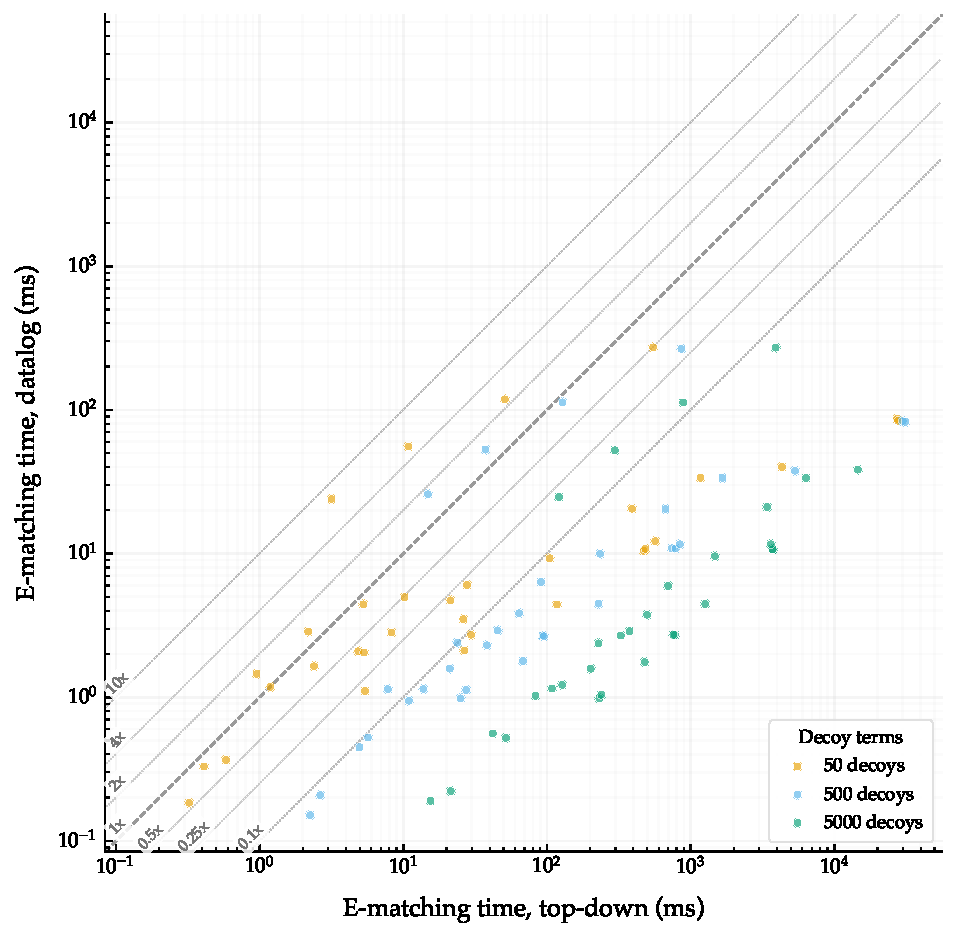
\includegraphics[width=\linewidth]{figs/matcher_cost_synthetic.pdf}
    \caption{Synthetic benchmarks.}
    \label{fig:matcher-cost-synthetic}
  \end{subfigure}\hfill
  \begin{subfigure}[t]{0.48\textwidth}
    \centering
    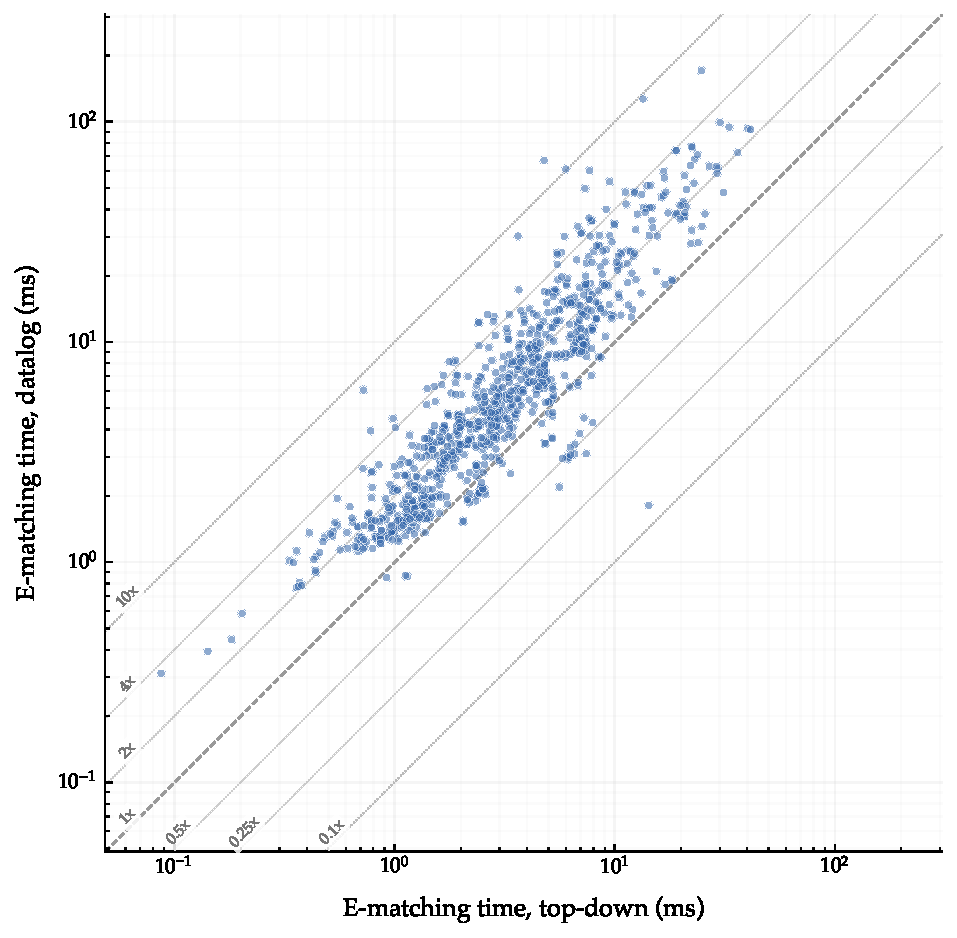
\includegraphics[width=\linewidth]{figs/matcher_cost_verus.pdf}
    \caption{Verus benchmarks.}
    \label{fig:matcher-cost-verus}
  \end{subfigure}
  \caption{Per-query e-matching time, top-down (x-axis) versus relational
  (y-axis), in seconds. Points below the diagonal are queries on which
  relational e-matching is faster. Left: synthetic benchmarks designed to
  stress nested patterns. Right: queries from the Verus program verifier.}
  \label{fig:matcher-cost}
\end{figure*}

We focus on e-matching time in isolation, rather than end-to-end solve time as
our current relational e-matching implementation is a prototype with significant
overhead from the \texttt{im::OrdMap} data structure. Thus, given a 60s timeout,
we the relation e-matching approach solves 96 queries (75 \%) on synthetic
benchmarks and 2247 queries (59.7 \%) on Verus benchmarks, while the top-down
approach solves 123 queries (96.1 \%) on synthetic benchmarks and 2414 queries (64.2
\%) on Verus benchmarks. We discuss the end-to-end picture in more detail in
Section~\ref{sec:conclusion}.

\subsection{Synthetic benchmarks}

The synthetic suite is a parameterized generalization of the running example
from Section~\ref{sec:background}. Each query uses a nested trigger similar to
\smt{g(h(x), x)}, but could also vary in the number 

We populate the e-graph with a varying number of
\emph{decoy} entries: extra ground assertions of the form \smt{(g d_i d_i)}
that add to the \smt{g}-table without contributing to any match. The number
of decoys is the principal axis of variation; a smaller axis varies the size
of the \smt{h}-table. Decoys exercise precisely the asymmetry that
distinguishes the two algorithms: top-down e-matching must scan every
\smt{g}-entry (decoys included) to find candidates, whereas relational
e-matching starts from the comparatively small \smt{h}-table and
index-joins into \smt{g}, touching only the relevant entries. The suite is
therefore designed to reward the relational approach as the decoy count
grows.

On this suite, relational e-matching is dramatically faster than top-down
e-matching. Of the 94 queries solved by both matchers, relational e-matching is
faster on 87, with a median speedup of $25\times$ ($2.92\times$ mean). Additionally,
the speedup grows with the number of decoys, as expected. 

\subsection{Verus benchmarks}

 Restricting attention to
the $n = 908$ queries that complete within one second under both matchers
, top-down e-matching is faster on
average, with a median ratio of $1.77\times$ (mean $2.04\times$)
in favor of top-down; relational e-matching is faster on only $53$ of the
$908$ queries.

These results suggest that more work is needed to realize the asymptotic
advantage of relational e-matching does not translate directly into a practical
win on real workloads. Closing this gap is the central engineering challenge
identified in Section~\ref{sec:conclusion}.
